\documentclass{standalone}
\usepackage{tikz}
\usetikzlibrary{patterns, positioning}

\begin{document}
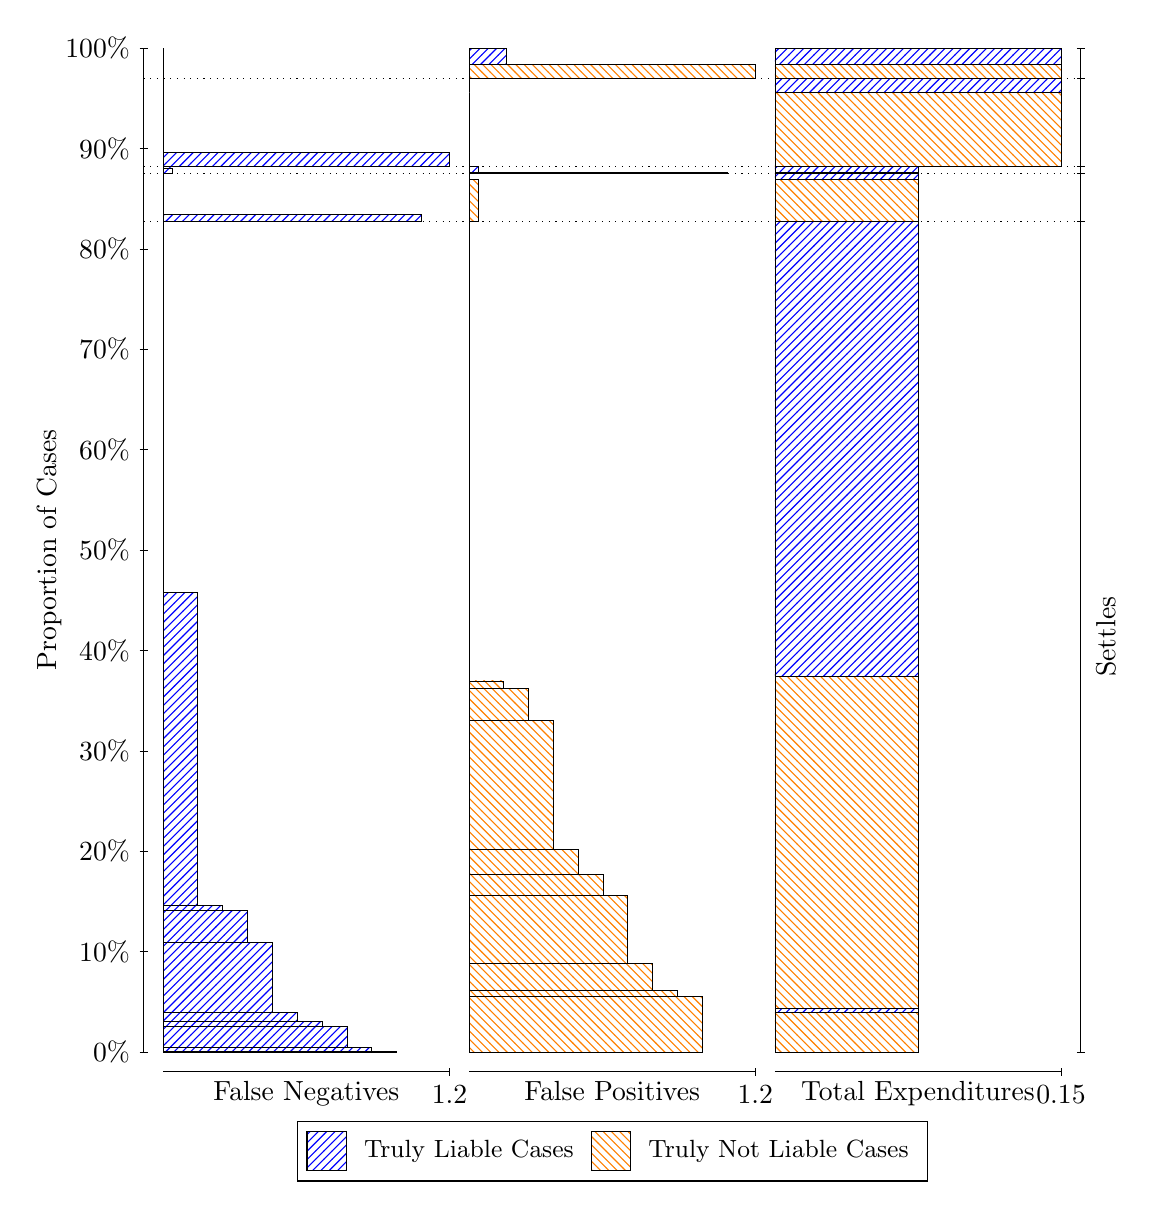
\begin{tikzpicture}
\draw[black, very thin] (1.5,1.75) -- (1.5,14.5);
\node[rotate=90, anchor=center] at (0.3, 8.125) {Proportion of Cases};
\draw[black, very thin] (1.45,1.75) -- (1.55,1.75);
\node[anchor=east] at (1.45, 1.75) {0\%};
\draw[black, very thin] (1.45,3.025) -- (1.55,3.025);
\node[anchor=east] at (1.45, 3.025) {10\%};
\draw[black, very thin] (1.45,4.3) -- (1.55,4.3);
\node[anchor=east] at (1.45, 4.3) {20\%};
\draw[black, very thin] (1.45,5.575) -- (1.55,5.575);
\node[anchor=east] at (1.45, 5.575) {30\%};
\draw[black, very thin] (1.45,6.85) -- (1.55,6.85);
\node[anchor=east] at (1.45, 6.85) {40\%};
\draw[black, very thin] (1.45,8.125) -- (1.55,8.125);
\node[anchor=east] at (1.45, 8.125) {50\%};
\draw[black, very thin] (1.45,9.4) -- (1.55,9.4);
\node[anchor=east] at (1.45, 9.4) {60\%};
\draw[black, very thin] (1.45,10.675) -- (1.55,10.675);
\node[anchor=east] at (1.45, 10.675) {70\%};
\draw[black, very thin] (1.45,11.95) -- (1.55,11.95);
\node[anchor=east] at (1.45, 11.95) {80\%};
\draw[black, very thin] (1.45,13.225) -- (1.55,13.225);
\node[anchor=east] at (1.45, 13.225) {90\%};
\draw[black, very thin] (1.45,14.5) -- (1.55,14.5);
\node[anchor=east] at (1.45, 14.5) {100\%};

\draw[black, very thin] (13.4,1.75) -- (13.4,14.5);
\draw[black, very thin] (13.35,1.75) -- (13.45,1.75);
\node[anchor=west] at (13.35, 1.75) {};
\draw[black, very thin] (13.35,12.299) -- (13.45,12.299);
\node[anchor=west] at (13.35, 12.299) {};
\draw[black, very thin] (13.35,12.911) -- (13.45,12.911);
\node[anchor=west] at (13.35, 12.911) {};
\draw[black, very thin] (13.35,12.993) -- (13.45,12.993);
\node[anchor=west] at (13.35, 12.993) {};
\draw[black, very thin] (13.35,14.117) -- (13.45,14.117);
\node[anchor=west] at (13.35, 14.117) {};
\draw[black, very thin] (13.35,14.5) -- (13.45,14.5);
\node[anchor=west] at (13.35, 14.5) {};

\draw[black, very thin, pattern color=blue, pattern=north east lines] (1.75,1.75) rectangle (4.712,1.7593);
\draw[black, very thin, pattern color=blue, pattern=north east lines] (1.75,1.7593) rectangle (4.396,1.8046);
\draw[black, very thin, pattern color=blue, pattern=north east lines] (1.75,1.8046) rectangle (4.0801,2.0731);
\draw[black, very thin, pattern color=blue, pattern=north east lines] (1.75,2.0731) rectangle (3.7641,2.1379);
\draw[black, very thin, pattern color=blue, pattern=north east lines] (1.75,2.1379) rectangle (3.4482,2.2543);
\draw[black, very thin, pattern color=blue, pattern=north east lines] (1.75,2.2543) rectangle (3.1322,3.1383);
\draw[black, very thin, pattern color=blue, pattern=north east lines] (1.75,3.1383) rectangle (2.8163,3.5512);
\draw[black, very thin, pattern color=blue, pattern=north east lines] (1.75,3.5512) rectangle (2.5004,3.6151);
\draw[black, very thin, pattern color=blue, pattern=north east lines] (1.75,3.6151) rectangle (2.1844,7.5859);
\draw[black, very thin, pattern color=orange, pattern=north west lines] (1.75,7.5859) rectangle (1.75,12.299);
\draw[black, very thin, pattern color=blue, pattern=north east lines] (1.75,12.299) rectangle (5.0279,12.383);
\draw[black, very thin, pattern color=orange, pattern=north west lines] (1.75,12.383) rectangle (1.75,12.911);
\draw[black, very thin, pattern color=blue, pattern=north east lines] (1.75,12.911) rectangle (1.8685,12.979);
\draw[black, very thin, pattern color=orange, pattern=north west lines] (1.75,12.979) rectangle (1.75,12.993);
\draw[black, very thin, pattern color=blue, pattern=north east lines] (1.75,12.993) rectangle (5.3833,13.176);
\draw[black, very thin, pattern color=orange, pattern=north west lines] (1.75,13.176) rectangle (1.75,14.117);
\draw[black, very thin, pattern color=orange, pattern=north west lines] (1.75,14.117) rectangle (1.75,14.296);
\draw[black, very thin, pattern color=blue, pattern=north east lines] (1.75,14.296) rectangle (1.75,14.5);
\draw[black, very thin, pattern color=orange, pattern=north west lines] (5.6333,1.75) rectangle (8.5953,2.4534);
\draw[black, very thin, pattern color=orange, pattern=north west lines] (5.6333,2.4534) rectangle (8.2793,2.5301);
\draw[black, very thin, pattern color=orange, pattern=north west lines] (5.6333,2.5301) rectangle (7.9634,2.871);
\draw[black, very thin, pattern color=orange, pattern=north west lines] (5.6333,2.871) rectangle (7.6475,3.7401);
\draw[black, very thin, pattern color=orange, pattern=north west lines] (5.6333,3.7401) rectangle (7.3315,4.0039);
\draw[black, very thin, pattern color=orange, pattern=north west lines] (5.6333,4.0039) rectangle (7.0156,4.3232);
\draw[black, very thin, pattern color=orange, pattern=north west lines] (5.6333,4.3232) rectangle (7.0156,4.3236);
\draw[black, very thin, pattern color=orange, pattern=north west lines] (5.6333,4.3236) rectangle (6.6996,5.9593);
\draw[black, very thin, pattern color=orange, pattern=north west lines] (5.6333,5.9593) rectangle (6.3837,6.3674);
\draw[black, very thin, pattern color=orange, pattern=north west lines] (5.6333,6.3674) rectangle (6.0678,6.4632);
\draw[black, very thin, pattern color=blue, pattern=north east lines] (5.6333,6.4632) rectangle (5.6333,12.299);
\draw[black, very thin, pattern color=orange, pattern=north west lines] (5.6333,12.299) rectangle (5.7518,12.827);
\draw[black, very thin, pattern color=blue, pattern=north east lines] (5.6333,12.827) rectangle (5.6333,12.911);
\draw[black, very thin, pattern color=orange, pattern=north west lines] (5.6333,12.911) rectangle (8.9112,12.925);
\draw[black, very thin, pattern color=blue, pattern=north east lines] (5.6333,12.925) rectangle (5.7518,12.993);
\draw[black, very thin, pattern color=orange, pattern=north west lines] (5.6333,12.993) rectangle (5.6333,13.934);
\draw[black, very thin, pattern color=blue, pattern=north east lines] (5.6333,13.934) rectangle (5.6333,14.117);
\draw[black, very thin, pattern color=orange, pattern=north west lines] (5.6333,14.117) rectangle (9.2667,14.296);
\draw[black, very thin, pattern color=blue, pattern=north east lines] (5.6333,14.296) rectangle (6.1072,14.5);
\draw[black, very thin, pattern color=orange, pattern=north west lines] (9.5167,1.75) rectangle (11.333,2.2539);
\draw[black, very thin, pattern color=blue, pattern=north east lines] (9.5167,2.2539) rectangle (11.333,2.3085);
\draw[black, very thin, pattern color=orange, pattern=north west lines] (9.5167,2.3085) rectangle (11.333,6.5178);
\draw[black, very thin, pattern color=blue, pattern=north east lines] (9.5167,6.5178) rectangle (11.333,12.299);
\draw[black, very thin, pattern color=orange, pattern=north west lines] (9.5167,12.299) rectangle (11.333,12.827);
\draw[black, very thin, pattern color=blue, pattern=north east lines] (9.5167,12.827) rectangle (11.333,12.911);
\draw[black, very thin, pattern color=orange, pattern=north west lines] (9.5167,12.911) rectangle (11.333,12.925);
\draw[black, very thin, pattern color=blue, pattern=north east lines] (9.5167,12.925) rectangle (11.333,12.993);
\draw[black, very thin, pattern color=orange, pattern=north west lines] (9.5167,12.993) rectangle (13.15,13.934);
\draw[black, very thin, pattern color=blue, pattern=north east lines] (9.5167,13.934) rectangle (13.15,14.117);
\draw[black, very thin, pattern color=orange, pattern=north west lines] (9.5167,14.117) rectangle (13.15,14.296);
\draw[black, very thin, pattern color=blue, pattern=north east lines] (9.5167,14.296) rectangle (13.15,14.5);
\draw[black, dotted] (1.5,12.299) -- (13.4,12.299);
\draw[black, dotted] (1.5,12.911) -- (13.4,12.911);
\draw[black, dotted] (1.5,12.993) -- (13.4,12.993);
\draw[black, dotted] (1.5,14.117) -- (13.4,14.117);
\draw[black, very thin] (1.75,1.5) -- (5.3833,1.5);
\node[anchor=north] at (3.5667, 1.5) {False Negatives};
\draw[black, very thin] (5.3833,1.45) -- (5.3833,1.55);
\node[anchor=north] at (5.3833, 1.45) {1.2};

\draw[black, very thin] (5.6333,1.5) -- (9.2667,1.5);
\node[anchor=north] at (7.45, 1.5) {False Positives};
\draw[black, very thin] (9.2667,1.45) -- (9.2667,1.55);
\node[anchor=north] at (9.2667, 1.45) {1.2};

\draw[black, very thin] (9.5167,1.5) -- (13.15,1.5);
\node[anchor=north] at (11.333, 1.5) {Total Expenditures};
\draw[black, very thin] (13.15,1.45) -- (13.15,1.55);
\node[anchor=north] at (13.15, 1.45) {0.15};

\node[black, centered, rotate=90] at (13.72, 7.0245) {Settles};





\draw (7.449999999999999,1.5) node[draw=none] (baseCoordinate) {};
\begin{scope}[align=center]
        \matrix[scale=0.5, draw=black, below=0.5cm of baseCoordinate, nodes={draw}, column sep=0.1cm]{
            \node[rectangle, draw, minimum width=0.5cm, minimum height=0.5cm, pattern=north east lines, pattern color=blue] {}; &
            \node[draw=none, font=\small] (B) {Truly Liable Cases}; &
            \node[rectangle, draw, minimum width=0.5cm, minimum height=0.5cm, pattern=north west lines, pattern color=orange] {}; &
            \node[draw=none, font=\small] (B) {Truly Not Liable Cases}; \\
            };
\end{scope}

\end{tikzpicture}
\end{document}